% !TeX root = ../../Book2.tex
% 纲要标题：### 16.2 相交数的构造
% 纲要位置：几何学计划纲要.md，第 1632 行。
% 正文状态：初稿；尚未正式审核。

% 纲要内容开始
% 
% * 互补维子流形的线性取向
% * 横截扰动与零维交集
% * 一参数族给出的配边
% * 交数与帽积配对的比较
% 
% 纲要内容结束

\section{相交数的构造}
\label{g2:sec:1602}

环面上的一条经线和一条纬线相交一次；把其中一条弯曲，可能额外出现两个交点，却仍不能把两条曲线彻底分开。记录每次穿过的方向后，新出现的两个交点符号相反，计数因而保持不变。第6章用杯积与基本类定义了代数配对，本节将证明，这个配对正是几何中的带符号交点数。先明确局部符号，再用横截扰动与一维配边处理不横截的情形，最后在管状邻域中核对帽积。

\subsection{互补维子流形的线性取向}
\label{g2:subsec:1602:01}

设 \(M\) 是已定向、无边界的光滑 \(n\) 维流形，\(A^p,B^q\subset M\) 是已定向、无边界的嵌入子流形，\(p+q=n\)。在横截交点 \(z\)，两个切空间互补，因此把它们的基接在一起，就能与环境定向比较。

\begin{definition}\label{g2:def:local-intersection-sign}
	在上述条件下，取 \(\mathrm{T}_zA\) 的正向基 \((a_1,\ldots,a_p)\) 和 \(\mathrm{T}_zB\) 的正向基 \((b_1,\ldots,b_q)\)。若
	\[
		(a_1,\ldots,a_p,b_1,\ldots,b_q)
	\]
	是 \(\mathrm{T}_zM\) 的正向基，定义局部相交符号 \(\varepsilon_z(A,B)=1\)；否则定义为 \(-1\)。若 \(A\pitchfork B\) 且 \(A\cap B\) 紧，定义其\term[xiangjiaoshu]{相交数}[intersection number]为
	\[
		I_M(A,B)=\sum_{z\in A\cap B}\varepsilon_z(A,B).
	\]
\end{definition}

更换两片的正向基只会乘上两个正行列式，所以符号与这些选择无关。横截逆像定理给出 \(\dim(A\cap B)=p+q-n=0\)，紧的零维流形是有限点集，因而上式是有限和。若 \(A\) 紧且 \(B\) 在 \(M\) 中闭，交集自动紧。维数为零的定向子流形按带符号的点理解，取向比较也包含这个符号。

\ProseParagraphBreak

为了把交点计数用于一般映射，需要把两片的比较改写为一个线性同构的符号。给法丛 \(\nu_MB=\mathrm{T}M|_B/\mathrm{T}B\) 取定向，使
\begin{equation}\label{g2:eq:normal-first-orientation}
	(\nu_MB,\mathrm{T}B)=\mathrm{T}M.
\end{equation}
这里法方向排在切方向之前：把一个法向基任意提升到环境切空间，再接上 \(B\) 的正向基，所得必须是环境的正向基。提升的改变只增加切向分量，不改变行列式。这个约定称为法向优先。

\begin{proposition}\label{g2:prop:intersection-linear-signs}
	在互补维横截交点处，商投影诱导的同构
	\[
		\mathrm{T}_zA\longrightarrow\nu_zB
	\]
	的定向符号等于 \(\varepsilon_z(A,B)\)。交换两片、反转一片定向及反转环境定向分别给出
	\[
		\varepsilon_z(B,A)=(-1)^{pq}\varepsilon_z(A,B),\qquad
		\varepsilon_z(-A,B)=-\varepsilon_z(A,B),\qquad
		\varepsilon_z^{\,-M}(A,B)=-\varepsilon_z^{\,M}(A,B).
	\]
	反转 \(B\) 的定向同样使符号反转。
\end{proposition}
\begin{proof}
	横截性及维数相等保证所列商映射为同构。相对于一个法向优先的环境基，把 \(A\) 的基分解为法向分量与切向分量；接上 \(B\) 的基后，矩阵为分块三角形，下方切向分量不影响行列式，符号就是法向分量矩阵的符号。交换两组基需要作 \(pq\) 次向量交换，得到 \((-1)^{pq}\)。反转任一基的定向或反转作为比较对象的环境定向，均改变一次符号。
\end{proof}

若 \(X^p\) 是已定向流形，\(f:X\to M\) 横截于 \(B\)，则在 \(x\in f^{-1}(B)\) 处定义
\[
	\varepsilon_x(f,B)=\operatorname{sgn}\bigl(\mathrm{T}_xX\xrightarrow{\mathrm{d}f_x}\mathrm{T}_{f(x)}M\longrightarrow\nu_{f(x)}B\bigr).
\]
当逆像紧时，令 \(I(f,B)=\sum_x\varepsilon_x(f,B)\)。这按源中的原像计数；不同源点即使映到同一个环境点，也分别贡献。嵌入 \(f=i_A\) 的情形正好恢复前面的定义。定义整数符号所需的是 \(X\) 的定向与 \(B\) 法丛的定向；环境及 \(B\) 的定向通过\eqref{g2:eq:normal-first-orientation}提供后者。若不选择这些定向，仍可取交点数模 \(2\)。

\begin{example}\label{g2:exm:torus-basic-intersection}
	在标准定向 \(\mathrm{d}x\wedge\mathrm{d}y\) 的环面 \(\mathbb R^2/\mathbb Z^2\) 中，令 \(a(t)=(t,0)\)、\(b(t)=(0,t)\)，参数均模 \(1\)。它们仅在原点相交，基 \((\partial_x,\partial_y)\) 正向，所以 \(I(a,b)=1\)、\(I(b,a)=-1\)。\(b\) 的正向法线是 \(\partial_x\)，而 \(a\) 的正向法线是 \(-\partial_y\)：后一个负号来自法向必须排在 \(\partial_x\) 之前。
\end{example}

\subsection{横截扰动与零维交集}
\label{g2:subsec:1602:02}

两片可能相切，甚至整段重合；此时直接数共同点不能得到一个稳定的数。横截性允许我们将其中一片略微移动。若用任意映射扰动，还需确认所得映射仍为嵌入。下面直接用环境微分同胚作扰动，整个过程都保持嵌入性质。

\begin{proposition}\label{g2:prop:transverse-embedded-perturbation}
	设 \(M\) 为无边界光滑流形，\(A\subset M\) 为紧无边界嵌入子流形，\(B\subset M\) 为闭的无边界嵌入子流形。对 \(A\) 的任意给定开邻域 \(\Omega\)，存在支撑于 \(\Omega\) 的、任意小的光滑环境同位 \(\Phi_t\)，使 \(\Phi_1(A)\pitchfork B\)。若两片维数互补，终点交集为有限点集。
\end{proposition}
\begin{proof}
	用有限张相对紧坐标图覆盖 \(A\)，其闭包包含于 \(\Omega\)。将各图的坐标向量场乘以紧支截断，再在图外补零，得到有限个紧支光滑场 \(V_1,\ldots,V_N\)，其值在 \(A\) 的每一点张成环境切空间。由\cref{g2:lem:uniformly-supported-evolution}，这些场的短时流 \(\varphi_j^s\) 都是环境微分同胚，并在同一个紧集外恒等。置
	\[
		\Psi(a,z)=\varphi_N^{a_N}\circ\cdots\circ\varphi_1^{a_1}(z),
		\qquad F(a,x)=\Psi(a,x),\quad x\in A.
	\]
	在 \(a=0\) 处，参数导数的像包含所有 \(V_j(x)\)，所以 \(F\) 的微分满射。\(A\) 紧，故可统一缩小参数球，使 \(F\) 在这个球乘 \(A\) 上均为淹没。\cref{g2:thm:parametric-transversality}于是给出任意小参数 \(a\)，使 \(F_a\pitchfork B\)。

	令 \(\Phi_t(z)=\Psi(ta,z)\)。每个时刻都是微分同胚，\(\Phi_0=\operatorname{id}\)，所以限制到 \(A\) 始终为嵌入。参数趋零时，这族映射及其各阶导数在共同紧支集上趋于恒等族，给出所需的小扰动。最后，\(\Phi_1(A)\) 紧，\(B\) 闭，故零维交集紧而有限。
\end{proof}

定向随 \(\Phi_t\) 推送给移动后的 \(A\)。由于环境微分同胚从恒等映射连续变化，它始终保持环境定向。对一般的 \(f:X\to M\)，其中 \(X\) 紧，\cref{g2:thm:relative-transversality}也给出与 \(f\) 同伦的横截扰动。下一小节将证明不同扰动所得的带符号和相同，之后便可将这个和定义为未必横截的 \(A,B\) 或 \(f,B\) 的相交数。

\begin{example}\label{g2:exm:intersection-birth-signs}
	在定向平面中，令 \(B\) 是沿正 \(x\) 方向的横轴，\(A_s\) 是按递增 \(x\) 定向的曲线 \(y=x^2-s\)。\(s<0\) 时局部没有交点；\(s>0\) 时交点为 \(x=\pm\sqrt{s}\)。两片切向量给出
	\[
		\det\begin{pmatrix}1&1\\2x&0\end{pmatrix}=-2x,
	\]
	故左交点的符号为 \(+1\)，右交点为 \(-1\)。两个新交点的总贡献为零。\(s=0\) 的相切切片没有局部横截符号，但整个参数族的交点轨迹 \(s=x^2\) 仍是一条光滑曲线。
\end{example}

\begin{figure}[htbp]
	\centering
	% !TeX root = ../Book2.tex
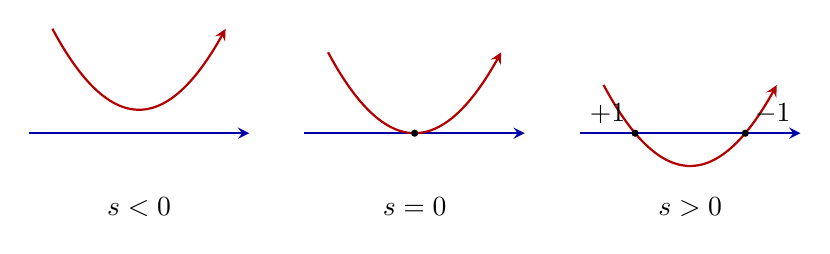
\begin{tikzpicture}[x=1cm,y=0.85cm,>=stealth]
	\begin{scope}
		\draw[->,blue!65!black,thick] (-1.4,0)--(1.4,0);
		\draw[->,red!70!black,thick,domain=-1.1:1.1,samples=40] plot (\x,{\x*\x+0.35});
		\node at (0,-1.1) {\(s<0\)};
	\end{scope}
	\begin{scope}[xshift=3.5cm]
		\draw[->,blue!65!black,thick] (-1.4,0)--(1.4,0);
		\draw[->,red!70!black,thick,domain=-1.1:1.1,samples=40] plot (\x,{\x*\x});
		\fill (0,0) circle (1.3pt);
		\node at (0,-1.1) {\(s=0\)};
	\end{scope}
	\begin{scope}[xshift=7cm]
		\draw[->,blue!65!black,thick] (-1.4,0)--(1.4,0);
		\draw[->,red!70!black,thick,domain=-1.1:1.1,samples=40] plot (\x,{\x*\x-0.49});
		\fill (-0.7,0) circle (1.3pt) node[above left] {\(+1\)};
		\fill (0.7,0) circle (1.3pt) node[above right] {\(-1\)};
		\node at (0,-1.1) {\(s>0\)};
	\end{scope}
\end{tikzpicture}

	\caption{相切附近的交点生成。曲线按横坐标递增定向，横轴向右定向；出现的两个交点分别贡献 \(+1\) 和 \(-1\)。}
	\label{g2:fig:intersection-pair}
\end{figure}

\subsection{一参数族给出的配边}
\label{g2:subsec:1602:03}

第14章已经将同伦横截化，得到连接端点逆像的紧流形。现在给这个配边定向，就能把模二不变性加强为整数不变性。这里需要核对时间方向与法方向的排列，而不只是指出端点成对出现。

\begin{theorem}\label{g2:thm:intersection-homotopy-invariance}
	设 \(M\) 是已定向、无边界的光滑 \(n\) 维流形，\(B\subset M\) 是已定向、闭的无边界嵌入 \(q\) 维子流形，\(X\) 是紧、已定向、无边界的光滑 \(p\) 维流形，\(p+q=n\)。若光滑映射 \(f_0,f_1:X\to M\) 横截于 \(B\) 且连续同伦，则
	\[
		I(f_0,B)=I(f_1,B).
	\]
\end{theorem}
\begin{proof}
	由\cref{g2:thm:transverse-homotopy-cobordism}，可选横截同伦 \(H:X\times[0,1]\to M\)，在两个端点的时间邻域中分别等于 \(f_0,f_1\)。其逆像 \(W=H^{-1}(B)\) 是紧一维带边界流形，边界是两端逆像的不交并。这里 \(X\) 紧、\(B\) 闭保证 \(W\) 紧。

	给 \(X\times[0,1]\) 取先 \(\mathrm{T}X\)、后 \(\partial_t\) 的乘积定向。商微分给出短正合列
	\[
		0\longrightarrow\mathrm{T}W\longrightarrow\mathrm{T}(X\times[0,1])|_W
		\xrightarrow{\ \overline{\mathrm{d}H}\ }H^*\nu B\longrightarrow0.
	\]
	规定 \(W\) 的正向，使法方向排在 \(W\) 的切方向之前，即 \((H^*\nu B,\mathrm{T}W)\) 给出源乘积的定向。更具体地，先列法基的提升，最后列 \(W\) 的正向切向量。

	在端点邻域，\(H\) 与时间无关。若 \(x\in f_i^{-1}(B)\)，记其局部符号为 \(\varepsilon_x\)。法基在 \(\mathrm{T}_xX\) 中的提升相对于 \(X\) 定向具有符号 \(\varepsilon_x\)，故上述规则使 \(W\) 的正向切向量为 \(\varepsilon_x\partial_t\)。采用外法向优先的边界定向，\(t=1\) 端点的符号是 \(\varepsilon_x\)，\(t=0\) 端点的符号是 \(-\varepsilon_x\)。因此
	\[
		\sum_{z\in\partial W}\varepsilon_z=I(f_1,B)-I(f_0,B).
	\]
	紧一维有向流形的边界符号之和为零：按第14章证明中的有限坐标弧分割，把各小弧沿定向排列，每条小弧贡献“终点减起点”，内部端点两两抵消，剩下的就是边界端点。于是右端为零。
\end{proof}

由此可对任意光滑 \(f:X\to M\) 选一个横截扰动 \(f'\)，定义 \(I(f,B)=I(f',B)\)。两个这样的扰动均与 \(f\) 同伦，定理保证良定义。对紧嵌入 \(A\) 使用上一小节的环境扰动，便定义 \(I_M(A,B)\)。其交换及反向规则仍成立：先把两片置于横截位置，再应用\cref{g2:prop:intersection-linear-signs}；更换所移动的一片也不影响结果，因为保持定向的环境微分同胚满足 \(I(A,\Phi(B))=I(\Phi^{-1}(A),B)\)，而 \(\Phi^{-1}|_A\) 与包含映射同伦。

\ProseParagraphBreak

紧性可以用“整个交点轨迹紧”替代，但不能只要求每张切片有有限个交点。例如 \(f_t:\mathbb R\to\mathbb R\)、\(f_t(x)=tx-1\)，以正向原点作为 \(B\)。\(t=0\) 时无交点，\(t>0\) 时恰有一个符号为正的交点 \(x=1/t\)。当 \(t\downarrow0\) 时它逃向无穷，轨迹不是紧配边，所以整数计数发生变化。这个例子说明，在非紧源上应用配边证明时，必须控制整条同伦的逆像。

\subsection{交数与帽积配对的比较}
\label{g2:subsec:1602:04}

以下设环境 \(M\) 闭且已定向，以便使用整数基本类 \([M]\)。\cref{g2:cor:closed-poincare-duality}给出同构
\[
	D_M:H^k(M;\mathbb Z)\longrightarrow H_{n-k}(M;\mathbb Z),\qquad
	D_M(\alpha)=\alpha\frown[M].
\]
对闭已定向嵌入子流形 \(i_B:B^q\hookrightarrow M\)，记
\[
	\mathrm{PD}_M(B)=D_M^{-1}\bigl((i_B)_*[B]\bigr)\in H^{n-q}(M;\mathbb Z).
\]
这里的 \(\mathrm{PD}\) 是 Poincaré 对偶类；它由帽积定义。要证明它检测穿过 \(B\) 的次数，需在 \(B\) 附近找到一个具体相对类，并核对其帽积正好留下 \(B\) 的基本类。

\begin{lemma}\label{g2:lem:normal-relative-class}
	设 \(M\) 是闭、已定向的光滑 \(n\) 维流形，\(B\subset M\) 是闭、已定向的嵌入 \(q\) 维子流形，\(p=n-q\)。法丛采用\eqref{g2:eq:normal-first-orientation}的定向。存在唯一的类
	\[
		u_B\in H^p(M,M\setminus B;\mathbb Z),
	\]
	使它在每个小法向 \(p\) 维盘上的限制，在正向局部基本类上取值 \(1\)。若 \(\overline u_B\) 是它在绝对上同调中的像，则
	\begin{equation}\label{g2:eq:normal-class-cap-fundamental}
		\overline u_B\frown[M]=(i_B)_*[B],\qquad
		\overline u_B=\mathrm{PD}_M(B).
	\end{equation}
\end{lemma}
\begin{proof}
	由\cref{g2:thm:tubular-neighborhood}，可将 \(B\) 的一个开邻域 \(U\) 识别为法丛的一个开圆盘丛；沿纤维径向重参数化，它与整个法丛 \(E\) 微分同胚，并保持零截面及纤维定向。\cref{g2:prop:relative-cohomology-exactness}的切除把 \(H^p(M,M\setminus B)\) 识别为 \(H^p(E,E\setminus B)\)。因此先在法丛中构造相对类。

	对任一法丛可平凡化的开集 \(V\subset B\)，选保持法向定向的平凡化，得到空间对
	\[
		(E|_V,E|_V\setminus V)\cong
		(\mathbb R^p\times V,(\mathbb R^p\setminus\{0\})\times V).
	\]
	相对 Eilenberg--Zilber 比较给出
	\begin{equation}\label{g2:eq:normal-low-degree-local}
		H^j(E|_V,E|_V\setminus V;\mathbb Z)\cong H^{j-p}(V;\mathbb Z).
	\end{equation}
	恢复这一计算的理由：\cref{g2:prop:cross-cup-evaluation}证明中的相对链比较将左侧链模型写成 \(C_*(\mathbb R^p,\mathbb R^p\setminus\{0\})\otimes C_*(V)\)。第一因子的同调只在 \(p\) 次为 \(\mathbb Z\)；由\cref{g2:lem:free-complex-splitting}，其圈边界序列可分裂为一个 \(\mathbb Z\) 加若干两项可缩复形，故它链同伦等价于仅在 \(p\) 次有 \(\mathbb Z\) 的复形。张量后再取 \(\operatorname{Hom}(-,\mathbb Z)\)，便得到上同调的次数平移。特别地，\(j<p\) 时左侧为零，\(j=p\) 时它由每个分支上的纤维取值唯一确定；全部取值为 \(1\) 的类就是正向纤维生成元与 \(1\in H^0(V)\) 的外积。

	这些局部类可以唯一粘合。取覆盖紧流形 \(B\) 的有限个丛平凡化开集，逐个取并。对两个开集 \(V,W\)，相对 Mayer--Vietoris 列包含
	\[
		H^{p-1}(E|_{V\cap W},E|_{V\cap W}\setminus(V\cap W))
		\longrightarrow H^p(E|_{V\cup W},E|_{V\cup W}\setminus(V\cup W))
	\]
	及其后的“限制到 \(V,W\)，再取交集上的差”两条箭头。这条列由相对小链模型的短正合列取对偶得到，和第6章使用的相对 Mayer--Vietoris 构造相同。归纳时，交集位于新加入的平凡化开集中，故\eqref{g2:eq:normal-low-degree-local}适用。其 \(p-1\) 次群为零，且两侧的 \(p\) 次局部类在交集上都以每根正向纤维的取值 \(1\) 为特征，所以差为零。正合性给出延拓的存在与唯一性。相同正合列也保持低于 \(p\) 次的消失，完成归纳。于是得到 \(u_B\)。改变管状邻域或平凡化后，纤维的局部取值不变，唯一性保证所取的是同一相对类。

	接着计算帽积。把 \(u_B\) 切除到 \(U\)，记作 \(u\)。\cref{g2:prop:relative-cap}给出
	\[
		z_U=u\frown[U]_B\in H_q(U;\mathbb Z),
	\]
	其中 \([U]_B\in H_n(U,U\setminus B;\mathbb Z)\) 是第6章的紧集基本类。令 \(r:U\to B\) 为管状收缩。要证明 \(r_*z_U=[B]\)，依\cref{g2:lem:compact-localization}，只需在每个 \(b\in B\) 核对其顶次局部值。

	在 \(b\) 附近选法向优先的乘积坐标 \((z,y)\in\mathbb R^p\times\mathbb R^q\)，其中 \(B\) 为 \(z=0\)。令 \(v_b\in H^q(B,B\setminus\{b\};\mathbb Z)\) 为在 \(B\) 的正向局部基本类上取值 \(1\) 的类。相对帽积的自然性及\eqref{g2:eq:cap-evaluation}在小链模型中的同一计算给出
	\begin{equation}\label{g2:eq:normal-cap-local-test}
		\left\langle v_b,\operatorname{loc}_b(r_*z_U)\right\rangle
		=\left\langle u\smile r^*v_b,[U]_{\{b\}}\right\rangle=1.
	\end{equation}
	说明这里的支集对应：\(u\) 的相对支集为 \(B\)，\(r^*v_b\) 的相对支集为法纤维 \(r^{-1}(b)\)，两者相交于 \(b\)。所以其相对杯积在 \(H^n(U,U\setminus\{b\})\) 中；局部化的基本类正是 \([U]_{\{b\}}\)。最后一个等号是\cref{g2:prop:local-cross-normalization}：先法向、后基底的两个正向局部生成元之积，在环境正向基本类上取值 \(1\)。某个因子为零维时，该计算退为点上乘法，结论相同。

	因此 \(r_*z_U\) 在每点的局部值都与 \([B]\) 相同，基本类的唯一性给出等式。将紧支相对类映入 \(M\)，帽积自然性又给出
	\[
		\overline u_B\frown[M]=(i_U)_*z_U
		=(i_B)_*r_*z_U=(i_B)_*[B].
	\]
	中间等式使用管状邻域沿纤维缩放到零截面的形变收缩。最后由 \(D_M\) 的单射性，\(\overline u_B=\mathrm{PD}_M(B)\)。
\end{proof}

这个相对类把“穿过 \(B\)”变成一个可以拉回的代数条件。法向小盘上的归一化决定每次横穿的贡献，上一证明中的帽积计算则保证它与第6章已经采用的对偶约定一致。

\begin{theorem}[几何相交与对偶配对]\label{g2:thm:geometric-intersection-pairing}
	设 \(M\) 是闭、已定向的光滑 \(n\) 维流形，\(B\subset M\) 是闭、已定向的嵌入 \(q\) 维子流形，\(X\) 是闭、已定向的光滑 \(p\) 维流形，\(p+q=n\)。若光滑映射 \(f:X\to M\) 横截于 \(B\)，且法丛采用法向优先定向，则
	\[
		\sum_{x\in f^{-1}(B)}\varepsilon_x(f,B)
		=\left\langle f^*\mathrm{PD}_M(B),[X]\right\rangle.
	\]
	对任意光滑 \(f\)，左侧采用横截扰动所定义的 \(I(f,B)\) 后，等式仍成立。特别地，若 \(A^p\subset M\) 也是闭已定向嵌入子流形，记 \([A]\)、\([B]\) 为其基本类在 \(M\) 中的推前，则
	\begin{equation}\label{g2:eq:intersection-cup-pairing}
		I_M(A,B)=\langle\mathrm{PD}_M(B),[A]\rangle
		=\langle\mathrm{PD}_M(A)\smile\mathrm{PD}_M(B),[M]\rangle.
	\end{equation}
\end{theorem}
\begin{proof}
	令 \(Z=f^{-1}(B)\)。它是有限点集。上一引理的相对类拉回为
	\[
		f^*u_B\in H^p(X,X\setminus Z;\mathbb Z).
	\]
	基本类的局部化与相对配对自然性给出
	\[
		\left\langle f^*\mathrm{PD}_M(B),[X]\right\rangle
		=\langle f^*u_B,[X]_Z\rangle
		=\sum_{x\in Z}\left\langle(f^*u_B)_x,[X]_x\right\rangle.
	\]
	最后一步在 \(Z\) 的互不相交小坐标邻域中切除；基本类限制到每点都为该点的正向局部类，所以有限直和中的每项系数都是 \(1\)。

	对 \(x\in Z\)，取 \(f(x)\) 附近的法向坐标 \(z:M\supset U\to\mathbb R^p\)。法向部分 \(z\circ f\) 在 \(x\) 的微分是定义 \(\varepsilon_x(f,B)\) 的线性同构。由逆函数定理，它在小邻域内为局部微分同胚，按其行列式符号将 \([X]_x\) 送到正向法盘基本类或其相反数。\(u_B\) 在这个正向法盘上取值 \(1\)，故每项恰等于 \(\varepsilon_x(f,B)\)。这证明横截情形。

	一般 \(f\) 的横截扰动 \(f'\) 与 \(f\) 同伦，所以它们诱导相同的上同调拉回；左侧按此前的不变性定义，等式随之成立。取 \(f=i_A\)，得到\eqref{g2:eq:intersection-cup-pairing}的第一个等式。第二个等式由帽积顺序决定：
	\[
		\begin{aligned}
		\langle\mathrm{PD}_M(B),[A]\rangle
		&=\langle\mathrm{PD}_M(B),\mathrm{PD}_M(A)\frown[M]\rangle\\
		&=\langle\mathrm{PD}_M(A)\smile\mathrm{PD}_M(B),[M]\rangle,
		\end{aligned}
	\]
	最后一行正是\eqref{g2:eq:cap-evaluation}。因此此处杯积先放 \(A\) 的对偶类，再放 \(B\) 的对偶类。
\end{proof}

\begin{corollary}\label{g2:cor:intersection-homological-invariance}
	闭已定向光滑 \(n\) 维流形中的互补维闭已定向嵌入子流形，其相交数只依赖整数同调类。它是这些类的双线性配对；若任一类为挠类，则相交数为零。交换两类乘以 \((-1)^{pq}\)，反转任一子流形或环境的定向均使相交数反号。
\end{corollary}
\begin{proof}
	\(D_M^{-1}\)、杯积及基本类取值均线性，所以\eqref{g2:eq:intersection-cup-pairing}只依赖同调类且双线性。若 \(r[A]=0\)，则 \(rI_M(A,B)=0\)，而整数群无挠，故 \(I_M(A,B)=0\)，另一因子同理。对偶类次数分别为 \(q,p\)，分次交换律给出 \((-1)^{pq}\)。子流形反向使其基本类及对偶类反号；环境反向使 \([M]\) 与 \(D_M\) 都反号，因此两个对偶类各反号，最终的基本类取值再反号，总变化仍为负号。
\end{proof}

\begin{example}\label{g2:exm:torus-poincare-sign-check}
	回到环面中的 \(a,b\)。令 \(\xi,\eta\in H^1(T^2;\mathbb Z)\) 分别从第一、第二圆周拉回正向生成元，则 \(\langle\xi\smile\eta,[T^2]\rangle=1\)。由帽积取值公式，\(D(\xi)=[b]\)、\(D(\eta)=-[a]\)，故
	\[
		\mathrm{PD}(a)=-\eta,\qquad \mathrm{PD}(b)=\xi,\qquad
		\langle(-\eta)\smile\xi,[T^2]\rangle=1.
	\]
	这与两条正向曲线的实际交点符号相同，也说明法向优先约定中的负号如何与杯积交换符号配合。
\end{example}

式\eqref{g2:eq:intersection-cup-pairing}也对任意互补维同调类定义代数相交配对；当类已有光滑子流形代表时，定理将它解释为横截交点数。以 \(\mathbb F_2\) 为系数时，同样的局部类、粘合与帽积证明给出模二相交配对：局部生成元没有正负之分，因而不需要环境及两片的整数定向。
